\definecolor{biascolor}{rgb}{0.75,0.15,0.15}
\definecolor{robustcolor}{rgb}{0.15,0.50,0.75}
\definecolor{privacycolor}{rgb}{0.50,0.15,0.70}
\definecolor{safetycolor}{rgb}{0.10,0.60,0.20}

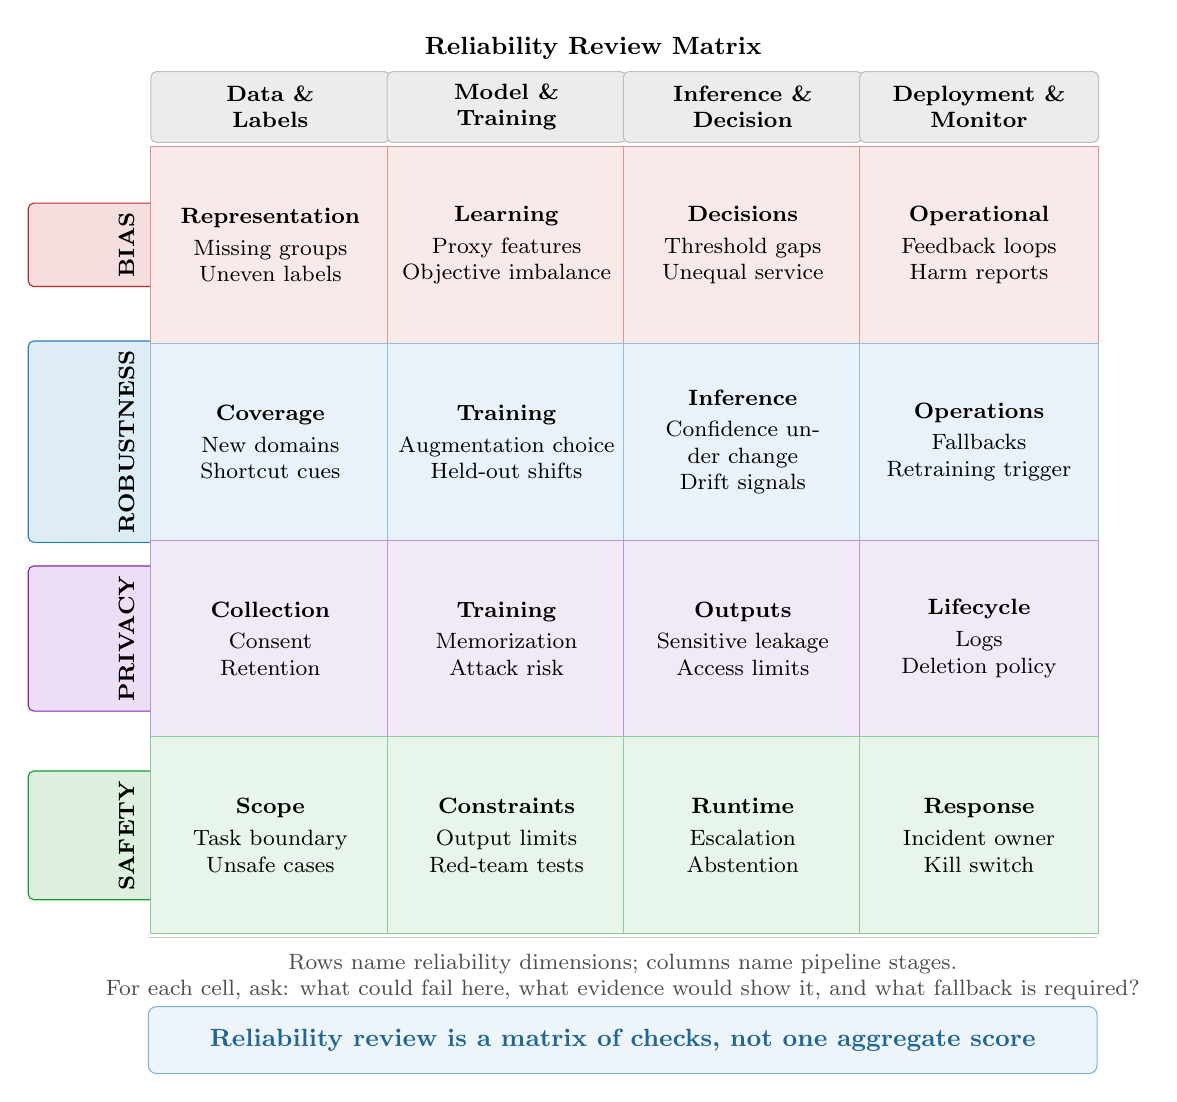
\begin{tikzpicture}[
    x=1cm, y=1cm,
    font=\small,
    %% Column centres:  x = 2.3  5.3  8.3  11.3   (cell width=3.0cm, pitch=3.0cm)
    %% Row centres:     y = 8.5  6.0  3.5   1.0   (row pitch=2.5cm)
    chdr/.style={draw=gray!50, fill=gray!15, rounded corners=2pt,
                 minimum width=3.0cm, minimum height=0.9cm,
                 text width=2.8cm, align=center, font=\footnotesize\bfseries},
    rhdr/.style={draw=gray!50, fill=gray!15, rounded corners=2pt,
                 minimum width=0.95cm, minimum height=2.5cm,
                 align=center, font=\footnotesize\bfseries, rotate=90},
    cell/.style={draw=gray!40, minimum width=3.0cm, minimum height=2.5cm,
                 text width=2.8cm, align=center, font=\footnotesize},
    bcell/.style={cell, fill=biascolor!10,    draw=biascolor!50},
    rcell/.style={cell, fill=robustcolor!10,  draw=robustcolor!50},
    pcell/.style={cell, fill=privacycolor!10, draw=privacycolor!50},
    scell/.style={cell, fill=safetycolor!10,  draw=safetycolor!50},
]

%% ── Title ────────────────────────────────────────────────────────────────
\node[font=\small\bfseries] at (6.4,11.0)
    {Reliability Review Matrix};

%% ── Column headers ───────────────────────────────────────────────────────
\node[chdr] at (2.3, 10.25)  {Data \&\\Labels};
\node[chdr] at (5.3, 10.25)  {Model \&\\Training};
\node[chdr] at (8.3, 10.25)  {Inference \&\\Decision};
\node[chdr] at (11.3,10.25)  {Deployment \&\\Monitor};

%% ── Row headers ──────────────────────────────────────────────────────────
\node[rhdr, fill=biascolor!15,    draw=biascolor]    at (0.475,8.5) {\textbf{BIAS}};
\node[rhdr, fill=robustcolor!15,  draw=robustcolor]  at (0.475,6.0) {\textbf{ROBUSTNESS}};
\node[rhdr, fill=privacycolor!15, draw=privacycolor] at (0.475,3.5) {\textbf{PRIVACY}};
\node[rhdr, fill=safetycolor!15,  draw=safetycolor]  at (0.475,1.0) {\textbf{SAFETY}};

%% ═══════════════════════════════════════════════════════════════════════════
%% BIAS ROW  (y = 8.5)
%% ═══════════════════════════════════════════════════════════════════════════
\node[bcell] at (2.3,8.5)
    {\textbf{Representation}\\[2pt]
     Missing groups\\Uneven labels};

\node[bcell] at (5.3,8.5)
    {\textbf{Learning}\\[2pt]
     Proxy features\\Objective imbalance};

\node[bcell] at (8.3,8.5)
    {\textbf{Decisions}\\[2pt]
     Threshold gaps\\Unequal service};

\node[bcell] at (11.3,8.5)
    {\textbf{Operational}\\[2pt]
     Feedback loops\\Harm reports};

%% ═══════════════════════════════════════════════════════════════════════════
%% ROBUSTNESS ROW  (y = 6.0)
%% ═══════════════════════════════════════════════════════════════════════════
\node[rcell] at (2.3,6.0)
    {\textbf{Coverage}\\[2pt]
     New domains\\Shortcut cues};

\node[rcell] at (5.3,6.0)
    {\textbf{Training}\\[2pt]
     Augmentation choice\\Held-out shifts};

\node[rcell] at (8.3,6.0)
    {\textbf{Inference}\\[2pt]
     Confidence under change\\Drift signals};

\node[rcell] at (11.3,6.0)
    {\textbf{Operations}\\[2pt]
     Fallbacks\\Retraining trigger};

%% ═══════════════════════════════════════════════════════════════════════════
%% PRIVACY ROW  (y = 3.5)
%% ═══════════════════════════════════════════════════════════════════════════
\node[pcell] at (2.3,3.5)
    {\textbf{Collection}\\[2pt]
     Consent\\Retention};

\node[pcell] at (5.3,3.5)
    {\textbf{Training}\\[2pt]
     Memorization\\Attack risk};

\node[pcell] at (8.3,3.5)
    {\textbf{Outputs}\\[2pt]
     Sensitive leakage\\Access limits};

\node[pcell] at (11.3,3.5)
    {\textbf{Lifecycle}\\[2pt]
     Logs\\Deletion policy};

%% ═══════════════════════════════════════════════════════════════════════════
%% SAFETY ROW  (y = 1.0)
%% ═══════════════════════════════════════════════════════════════════════════
\node[scell] at (2.3,1.0)
    {\textbf{Scope}\\[2pt]
     Task boundary\\Unsafe cases};

\node[scell] at (5.3,1.0)
    {\textbf{Constraints}\\[2pt]
     Output limits\\Red-team tests};

\node[scell] at (8.3,1.0)
    {\textbf{Runtime}\\[2pt]
     Escalation\\Abstention};

\node[scell] at (11.3,1.0)
    {\textbf{Response}\\[2pt]
     Incident owner\\Kill switch};

%% ══════════════════════════════════════════════════════════════════════════
%% LEGEND
%% ══════════════════════════════════════════════════════════════════════════
\draw[gray!40] (0.75,-0.3) -- (12.8,-0.3);
\node[font=\footnotesize, align=center, text=black!70] at (6.775,-0.8)
    {Rows name reliability dimensions; columns name pipeline stages.\\For each cell, ask: what could fail here, what evidence would show it, and what fallback is required?};

%% ── Key insight ──────────────────────────────────────────────────────────
\node[draw=robustcolor!60, rounded corners=3pt, fill=robustcolor!8,
      minimum width=12.05cm, minimum height=0.85cm, align=center,
      font=\small] at (6.775,-1.6)
    {\textcolor{robustcolor!80!black}{\bfseries
     Reliability review is a matrix of checks, not one aggregate score}};

\end{tikzpicture}
